\documentclass{article} 

\usepackage[polish]{babel}
\usepackage[utf8]{inputenc}
\usepackage[T1]{fontenc}

\usepackage{graphicx,color} %include pdf's (and png's for raster graphics... avoid raster graphics!) 

\usepackage{url} 

\usepackage[pdftex,hyperfootnotes=false,pdfborder={0 0 0}]{hyperref} %za wszystkimi pakietami; pdfborder nie wszedzie tak samo zaimplementowane bo specyfikacja nieprecyzyjna; pod miktex'em po prostu nie widac wtedy ramek


% Zmiana rozmiarów strony tekstu
\addtolength{\voffset}{-1cm}
\addtolength{\hoffset}{-1cm}
\addtolength{\textwidth}{2cm}
\addtolength{\textheight}{2cm}

%bardziej zyciowe parametry sterujace rozmieszczeniem rysunkow
\renewcommand{\topfraction}{.85}
\renewcommand{\bottomfraction}{.7}
\renewcommand{\textfraction}{.15}
\renewcommand{\floatpagefraction}{.66}
\renewcommand{\dbltopfraction}{.66}
\renewcommand{\dblfloatpagefraction}{.66}
\setcounter{topnumber}{9}
\setcounter{bottomnumber}{9}
\setcounter{totalnumber}{20}
\setcounter{dbltopnumber}{9}

% w³asny bullet list z malymi odstepami
\newenvironment{tightlist}{
\begin{itemize}
  \setlength{\itemsep}{1pt}
  \setlength{\parskip}{0pt}
  \setlength{\parsep}{0pt}}
{\end{itemize}}

%obrazkow szukamy w nastepujacym katalogu:
\graphicspath{{pics/}}



%\title{Sprawozdanie z laboratorium:\\Metaheurystyki i Obliczenia Inspirowane Biologicznie}
%\author{}
%\date{}


\begin{document}

%\input{_tytulowa} %dodaje zewnętrzny plik tex


\thispagestyle{empty} %bez numeru strony

\begin{center}

	{\large{Sprawozdanie z laboratorium:\\
	Komunikacja człowiek komputer}}

	\vspace{6ex}

	{\footnotesize\today}

\end{center}


\vspace{10ex}

Prowadzący: dr hab. inż. Maciej Komosiński

\vspace{5ex}

Autor:
\begin{tabular}{lllr}
\textbf{Radosław Osten} & inf106520 & grupa i3 & radek.osten@gmail.com \\
\end{tabular}

\vspace{5ex}

Zajęcia: środa, 18:30.


\newpage





\section{Wstep}

Teskt haha
$\Delta_{dir}$ wartosci $p_{dir}$ dla kata $90^\circ$.



\begin{figure}[!ht]
\begin{center}
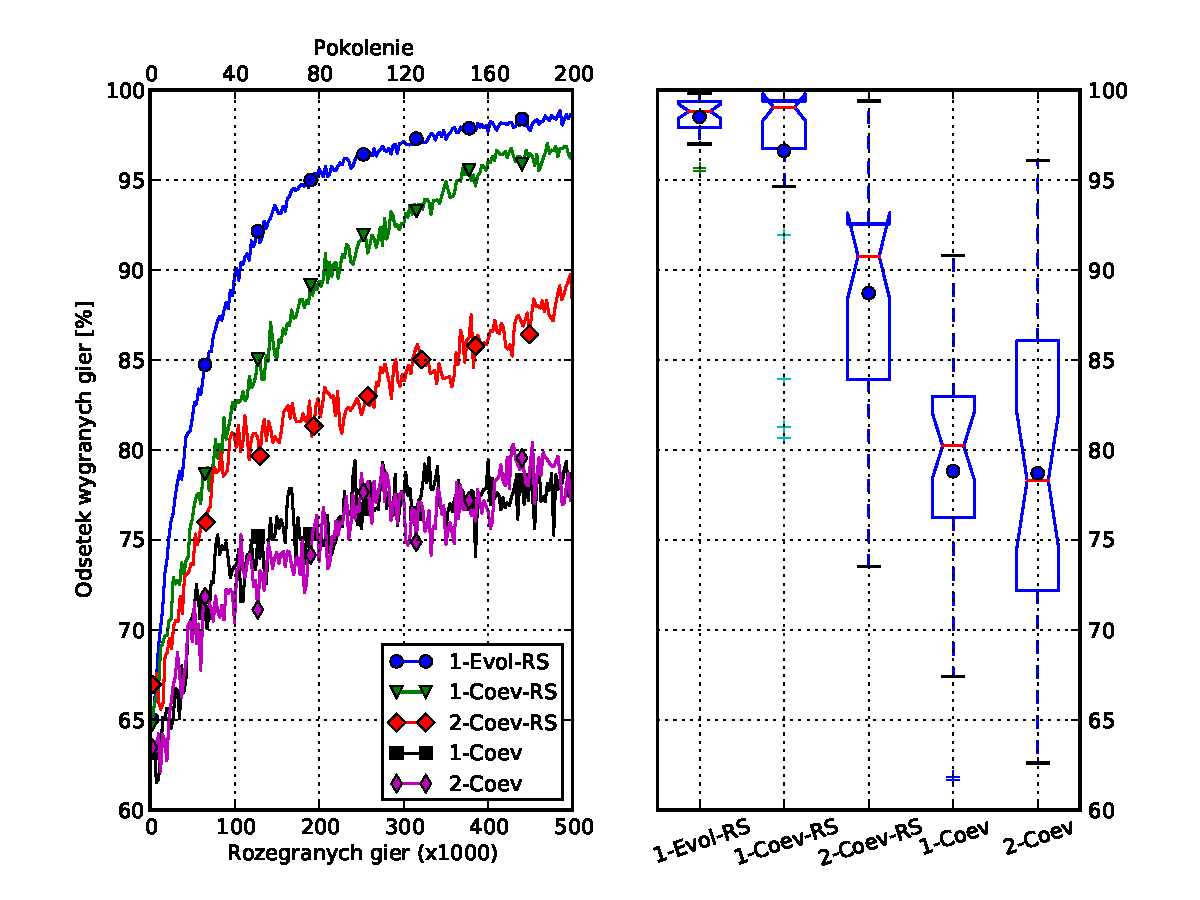
\includegraphics[width=1.15\textwidth]{myplot.pdf}
\end{center}
\caption{Podpis pod rysunkiem}
\label{fig-schemat}
\end{figure}


Lista:

\begin{tightlist}
\item wstawic schemat stworzony graphviz'em (Rys.~\ref{fig-schemat}),
\item test
\item odwolywac sie do rysunków, cytowan i czesci sprawozdania (np.\ rozdzial~\ref{sec-eksperymenty}).
\end{tightlist}


Przypis na dole strony \footnote{Poszukaj w Wikipedii hasa \emph{Dywiz}.}



\clearpage %pozwol umiescic zalegle rysunki od razu tutaj 


\section{Eksperymenty}
\label{sec-eksperymenty}

Tekst

\subsection{Cechy dobrego sprawozdania}

Kolejny tekst \cite{norman}


%%%%%%%%%%%%%%%% literatura %%%%%%%%%%%%%%%%

%\bibliography{sprawozd}
%\bibliographystyle{plain}

\begin{thebibliography}{1}

\bibitem{notes} John W. Dower {\em Readings compiled for History
  21.479.}  1991.

\bibitem{impj}  The Japan Reader {\em Imperial Japan 1800-1945} 1973:
  Random House, N.Y.

\bibitem{norman} E. H. Norman {\em Japan's emergence as a modern
  state} 1940: International Secretariat, Institute of Pacific
  Relations.

\bibitem{fo} Bob Tadashi Wakabayashi {\em Anti-Foreignism and Western
  Learning in Early-Modern Japan} 1986: Harvard University Press.

\end{thebibliography}


\end{document}

